\chapter{Comunicação SPI}\label{cap:com_spi}

A interface periférica serial (SPI) permite comunicação serial \textit{half/ full-duplex}, síncrona, com dispositivos externos. A interface pode ser configurada como mestre, caso em que fornece o sinal de relógio da comunicação (SCK) ao dispositivo externo escravo (\textit{slave}). A interface também é capaz de operar em configuração \textit{multimaster}.
Pode ser usada para uma variedade de propósitos, inclusive transferências síncronas simplex em duas linhas com uma possível linha de dados bidirecional ou comunicação confiável usando checagem CRC.
Normalmente, o SPI se conecta a dispositivos externos por 4 pinos:
\begin{itemize}
\item MISO: (\textit{Master In / Slave Out}) Esse pino é usado para transmitir dados do escravo para o mestre, no caso, do módulo de transmissão para o módulo de controle.
\item MOSI: (\textit{Master Out / Slave In}) Esse pino é usado para transmitir dados do mestre para o escravo, no caso, do módulo de controle para o módulo de transmissão.
\item SCK: (\textit{Serial Clock}) Esse pino é saída para o mestre e entrada para o escravo. É o sinal que determina a que instante os bits serão lidos
\item NSS: (\textit{Negated Slave Select}). Às vezes chamado de CSN, é um pino opcional para selecionar um dispositivo escravo, quando em nível baixo. Permite ao mestre do SPI comunicar-se com diversos escravos individualmente e evitar disputa pelas linhas de dados. Para este caso, foi usado um pino de um dos periféricos GPIO (\textit{General Purpose Input/Output} – Entrada/Saída de Propósito Geral) do módulo de controle, que foi configurado como saída.
\end{itemize}

Os pinos MOSI do mestre e do escravo são conectados, assim como os pinos MISO. Dessa forma, os dados são transferidos serialmente entre mestre e escravo (o bit mais significativo primeiro).
A comunicação é sempre iniciada pelo mestre. Quando o mestre transmite dados para um escravo através do pino MOSI, o escravo responde através do pino MISO. Isso implica uma comunicação \textit{full-duplex} com dados de saída e de entrada sincronizados pelo mesmo sinal de relógio (provido pelo mestre através do pino SCK).
A Figura~\ref{fig:spi} ilustra o processo de comunicação com um mestre e um escravo.

\begin{figure}
	\centering
	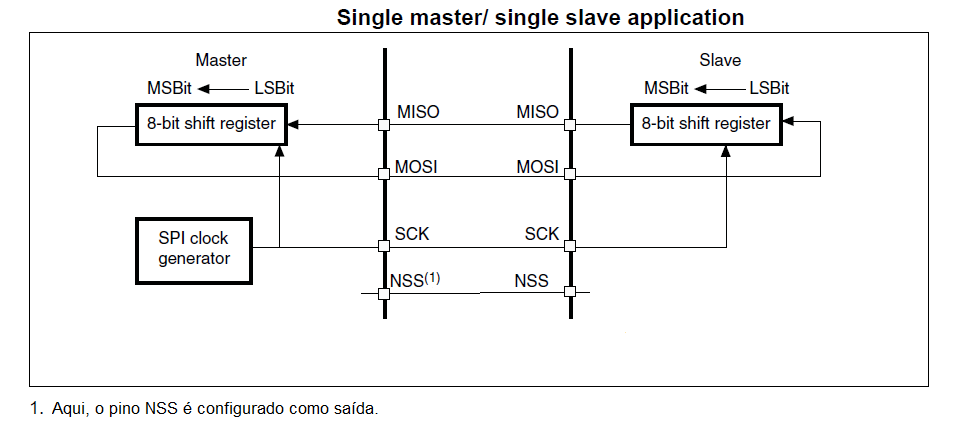
\includegraphics[scale=0.6]{SPI}
	\caption{Esquema da Comunicação SPI}
	\label{fig:spi}
\end{figure}

Para aprender a controlar a interface SPI do módulo de controle (mestre da comunicação), foram inicialmente feitos códigos em linguagem C, nos quais era feita a ativação do relógio do GPIO do pino NSS, configuração deste GPIO, a configuração dos registradores do periférico de SPI da \textit{Discovery} e o envio de comandos para leitura de registradores do NRF24.
Após isso, foi feita a biblioteca, em C, para comunicação SPI para este microcontrolador, tendo sempre o manual de referência da \textit{STMicroelectronics\textsuperscript{\textregistered}}\cite{stm32f4referencemanual} como guia.

% Ramificação constante ou taxa constante

% vim: tw=80 et ts=2 sw=2 sts=2 ft=tex spelllang=pt_br,en
